\documentclass[11pt,a4paper]{article}
\usepackage{amsmath,amsthm,amsfonts,amssymb,amscd}
\usepackage{enumerate} 
\usepackage{physics}
\usepackage{enumerate}
\usepackage{fancyhdr}
 \usepackage{hyperref}
\hypersetup{colorlinks,
    linkcolor=blue,
    citecolor=blue,      
    urlcolor=blue,
}
\usepackage{graphicx}


\oddsidemargin0.1cm 
\evensidemargin0.8cm
\textheight22.7cm 
\textwidth15cm \topmargin-0.5cm

\newtheorem{theorem}{Theorem}[section]
\newtheorem{lemma}[theorem]{Lemma}

\usepackage{listings}
\usepackage{xcolor}

\definecolor{codegreen}{rgb}{0,0.6,0}
\definecolor{codegray}{rgb}{0.5,0.5,0.5}
\definecolor{codepurple}{rgb}{0.58,0,0.82}
\definecolor{backcolour}{rgb}{0.95,0.95,0.92}

\lstdefinestyle{mystyle}{
    backgroundcolor=\color{backcolour},   
    commentstyle=\color{codegreen},
    keywordstyle=\color{magenta},
    numberstyle=\tiny\color{codegray},
    stringstyle=\color{codepurple},
    basicstyle=\ttfamily\footnotesize,
    breakatwhitespace=false,         
    breaklines=true,                 
    captionpos=b,                    
    keepspaces=true,                 
    numbers=left,                    
    numbersep=5pt,                  
    showspaces=false,                
    showstringspaces=false,
    showtabs=false,                  
    tabsize=2
}

\lstset{style=mystyle}

\newcommand{\silvia}[1]{{ {\color{blue}{(silvia)~#1}}}}
\newcommand{\grace}[1]{{ {\color{purple}{(grace)~#1}}}}

\newcommand{\MultiSet}{\mathrm{MultiSet}}
\newcommand{\len}{\mathrm{len}}
\newcommand{\din}{\texttt{d\_in}}
\newcommand{\dout}{\texttt{d\_out}}
\newcommand{\T}{\texttt{T} }
\newcommand{\F}{\texttt{F} }
\newcommand{\Relation}{\texttt{Relation}}
\newcommand{\X}{\mathcal{X}}
\newcommand{\Y}{\mathcal{Y}}
\newcommand{\True}{\texttt{True}}
\newcommand{\False}{\texttt{False}}
\newcommand{\clamp}{\texttt{clamp}}
\newcommand{\function}{\texttt{function}}
\newcommand{\float}{\texttt{float }}
\newcommand{\questionc}[1]{\textcolor{red}{\textbf{Question:} #1}}


\title{Privacy Proofs for OpenDP: Impute Constant Transformation}
\author{Grace Tian}
\date{Summer 2021}
\begin{document}


\maketitle
\tableofcontents

\section{Algorithm Implementation}
\subsection{Code in Rust}
The current OpenDP library contains the \texttt{make\_impute\_constant} function implementing the impute constant function. This is defined in lines 62-75 of the file \texttt{impute.rs} in the Git repository (\url{https://github.com/opendp/opendp/blob/21-impute/rust/opendp/src/trans/impute.rs#L62-L75}).

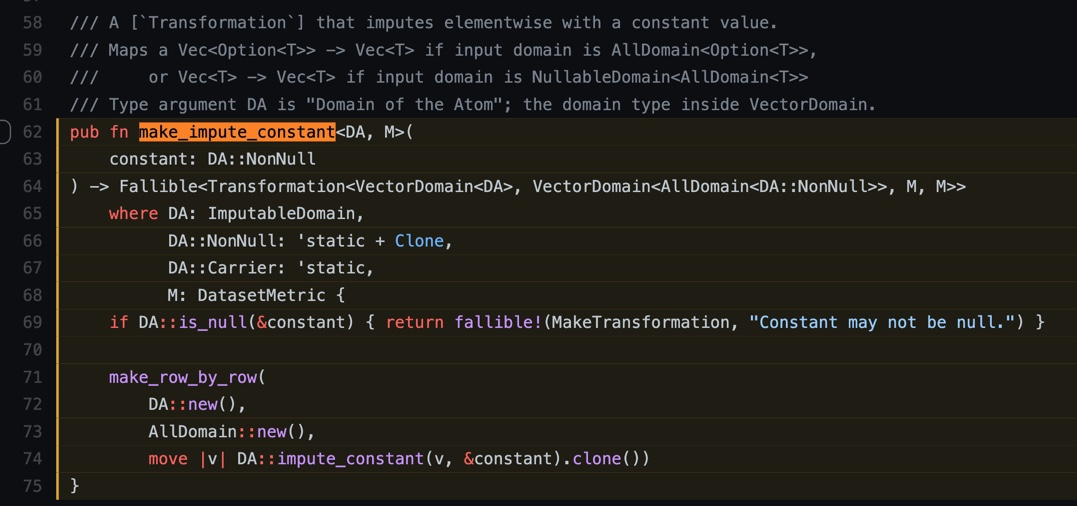
\includegraphics[width=\textwidth]{make_impute_constant.jpg}


\subsection{Pseudo Code in Python}\label{sec:pseudocode}

\subsubsection*{Preconditions}
To ensure the correctness of the output, we require the following preconditions:

\begin{itemize}
    \item \textbf{User-specified types:}
    \begin{itemize}
        \item Variable \texttt{\texttt{constant}} must be of type \texttt{DA::NonNull}
        \item Type \texttt{DA} must have traits \texttt{ImputableDomain} 
        \item \texttt{DA::NonNull} has traits \texttt{Clone}
    \end{itemize}
\end{itemize}

\subsubsection*{Postconditions}

\begin{itemize}
    \item Either a valid \texttt{Transformation} is returned or an error is returned.
\end{itemize}

\grace{Not sure if I need to include the error check for whether the constant is nonnull in line 69 code. Is it already checked? }
\begin{lstlisting}[language=Python,  escapechar=|]
def make_impute_constant(constant : DA::NonNull):
    input_domain = VectorDomain(DA);
    output_domain = VectorDomain(AllDomain(DA::NonNull));
    
    def Relation(d_in: u32, d_out: u32) -> bool: |\label{line:rel}|
        return d_out >= d_in*1

    def function(data: Vec(DA)) -> Vec(DA::NonNull): |\label{line:fn}|
        def impute_constant(x: DA) -> DA::NonNull:
            return constant if x.is_null else x
        return list(map(impute_constant, data)) |\label{line:map}|
        
    return Transformation(input_domain, output_domain, function(data?), input_metric, output_metric, stability_relation=Relation)

\end{lstlisting}

\grace{ Will need to change pseudocode so that it returns the result of a make row by row transformation (which the code does) instead of a Transformation directly. Make sure to ask.}

\subsection{Proof}
\begin{theorem}


For every setting of the input parameters \texttt{constant} to \texttt{make\_impute\_constant} such that the given preconditions hold, the transformation returned by \texttt{make\_impute\_constant} has the following properties:
\begin{enumerate}
    \item \textup{(Appropriate output domain).} If vector $v$ is in the \texttt{input\_domain}, then \texttt{function(v)} is in the \texttt{output\_domain}.
    \item \textup{(Domain-Metric Compatibility).} The domain \texttt{input\_domain} matches one of the possible domains listed in the definition of \texttt{input\_metric}, and likewise \texttt{output\_domain} matches one of the possible domains listed in the definition of \texttt{output\_metric}.
    \item \textup{(Stability Guarantee).} For every pair of elements $v, w$ in \texttt{input\_domain} and for every pair $(\din, \dout)$, where $\din$ is of the associated type for \texttt{input\_metric} and $\dout$ is the associated type for \texttt{output\_metric}, if $v,w$ are $d_{in}$-close under \texttt{input\_metric} and $\Relation(\din, \dout) = \True$, then $\function(v), \function(w)$ are $d_{out}$-close under \texttt{output\_metric}.
\end{enumerate}
\end{theorem}
\begin{proof}
\begin{enumerate}
\item \textbf{(Appropriate output domain).} 
In the case of \texttt{make\_impute\_constant}, this corresponds to showing that for every vector $v$ of elements of type \texttt{DA}, \texttt{function}$(v)$ is a vector of elements of type \texttt{DA::NonNull}.

The $\function(v)$ has type \texttt{Vec(DA)} follows from the assumption that element $v$ is in \texttt{input\_domain} and from the type signature of \texttt{function} in line~\ref{line:fn} of the pseudocode (Section~\ref{sec:pseudocode}), which takes in an element of type \texttt{Vec(DA)} and returns an element of type \texttt{Vec(DA::NonNull)}. If the Rust code compiles correctly, then the type correctness follows from the definition of the type signature enforced by Rust. Otherwise, the code raises an exception for incorrect input type. 

Lastly, we ensure that return type must be \texttt{NonNull} \grace{Attribute? Property? Carrier} \texttt{DA::NonNull} because we check to make sure the \texttt{constant} being imputed in the function must be null. \grace{Not sure if this needs to be explicit in the pseudo code with the error check, or if I can just cite some trait property.} This check already exists because in the input of the \texttt{make\_impute\_constant}, \texttt{constant} is required to have type of \texttt{DA::NonNull}.

\item \textbf{(Domain-metric compatibility).} The Symmetric distance is both the \texttt{input\_metric} and \texttt{output\_metric}.Symmetric distance is compatible with \texttt{VectorDomain(T)} for any generic type \texttt{T}, as stated in \href{https://www.overleaf.com/project/60d215bf90b337ac02200a99}{``List of definitions used in the pseudocode"}. The theorem holds because for \texttt{make\_impute\_constant}, the input domain is \texttt{VectorDomain(DA)} for generic type \texttt{TI} and the output domain is \texttt{VectorDomain(AllDomain(DA::NonNull))}. 

\item \textbf{(Stability guarantee).}     We know that $d_{in} \leq d_{out}$ because \texttt{Relation}($d_{in}$, $d_{out}$) $\texttt{ = True}$. Since the vectors $v, w$ are $d_{in}$-close, then $d_{Sym}(v, w) \leq d_{in}$.
    
    The function transformation just replaces the $\texttt{null}$ element in vectors $v$ and $w$ with \texttt{constant}. Since the null element is also counted toward the symmetric distance of the transformation, the symmetric distance of $\texttt{function}(v)$ and $\texttt{function}(w)$ stays the same. Therefore the transformation is $d_{out}$ close: $d_{sym}(\texttt{function}(v), \texttt{function}(w)) = d_{sym}(v, w) \leq d_{in} \leq d_{out}$

\end{enumerate}
\end{proof}

\end{document}
